\section{Introduction and fast Requirement Analysis}

%- Main user story --------------------------------- %
Since this is a small project with the aim to experiment something in \textit{Mobile Systems}, we never provide a detailed project with exhaustive analysis. However, we will give some important details by making a fast analysis.

\subsection{Main user story}

This \href{https://en.wikipedia.org/wiki/User_story}{\textit{user story}} shows the main description of the operation of the system:

\hspace{10pt}
\begin{center}
	\begin{userstory}[Main User Story]{us:main}
		The user:
		\begin{enumerate}
			\item uses his device and \textbf{opens the \gitberto application} on his mobile that \textbf{automatically connects with the paired physical robot}; 
			\item inserts a destination using the classical \textit{address searching} and the application shows the founded possibilities; then, \textbf{selects the desired target} to arrive to and the application calculates the route to get the destination;
			\item \textbf{clicks on the \textit{GO}} button;
			\item  \textbf{follows the physical \gitberto robot that started to move} guiding him towards the destination.
		\end{enumerate}
		
	\end{userstory}
\end{center}
\begin{figure}[h!]
	\centering
	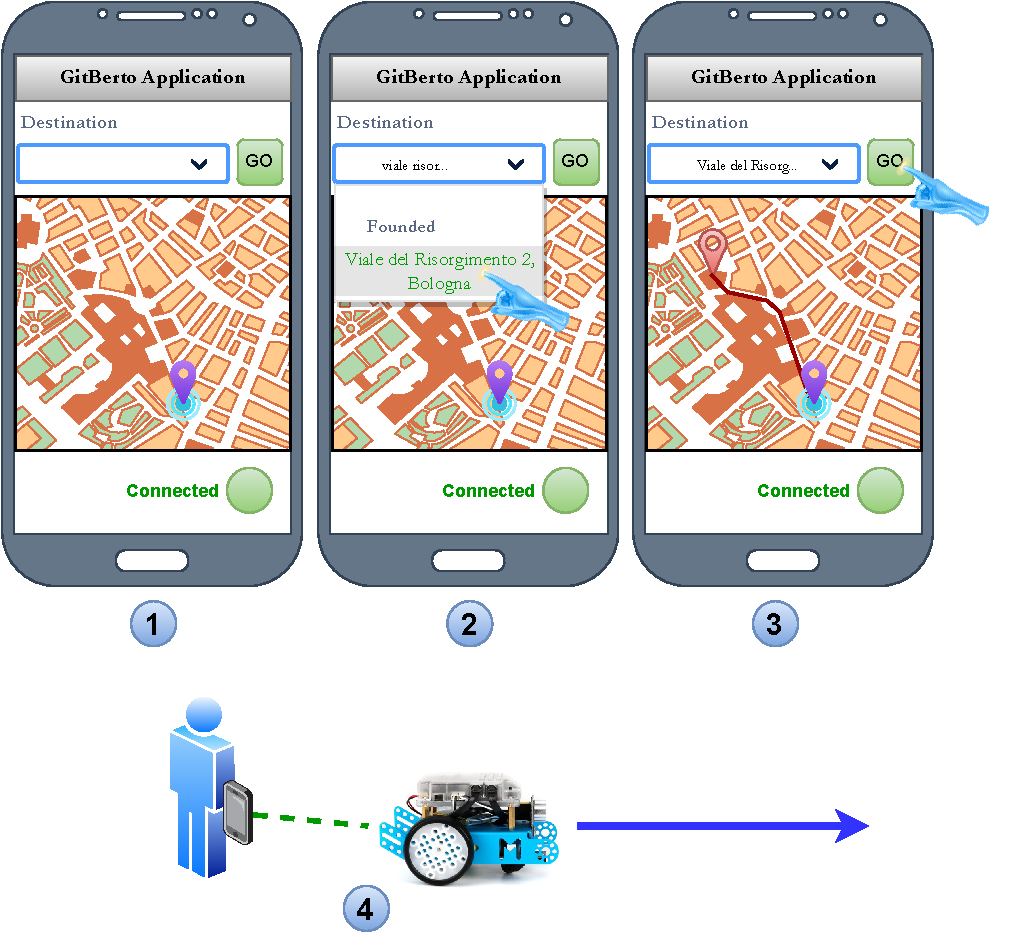
\includegraphics[width=0.7\textwidth]{img/user_story_main.pdf}
	\caption{Main user story representation}
	\label{fig:user_story_main}
\end{figure}

The figure \ref{fig:user_story_main} shows a graphical representation of the steps presented in the main user story.

\subsection{Main overview of the architecture of the system}

In order to simplify the work, we also make some \textbf{assumptions}:
\begin{enumerate}
	\item angle between routes are only right ($90\degree$);
	\item routes are all passable only by pedestrians;
	\item all others pedestrian shows the robot and avoid collisions with him;
	\item the position retrieved by the mobile device is exact without error.
\end{enumerate}

These assumptions let us concentrate with the main focus of this work without caring about others aspects that are mainly related with \href{https://en.wikipedia.org/wiki/Artificial_intelligence}{Artificial Intelligence}

As suggested by the assumption $3$, as a requirement \textbf{all the computation of positions and routes must be performed by the user device}. So, as expected, \textbf{the mobile device and the robot must communicate}, exchanging commands and data.

\begin{figure}[h!]
	\centering
	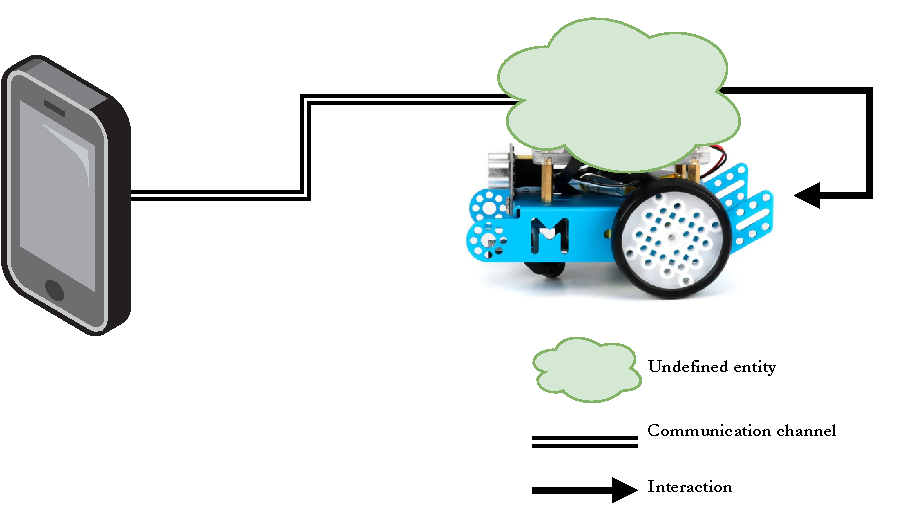
\includegraphics[width=0.8\textwidth]{img/coarse_architecture.pdf}
	\caption{\textit{Coarse} architecture of the system}
	\label{fig:coarse_architecture}
\end{figure}

The first \textit{coarse} architecture is shown by the figure \ref{fig:coarse_architecture} that only say that:
\begin{enumerate}
	\item there are two \textcolor{MidnightBlue}{\textbf{\textit{undefined entities}}} that are \textit{executable}: one on the device and the other on the robot;
	\item this two entities has a \textit{communication channel} that can be used for \textcolor{MidnightBlue}{\textbf{communication}};
	\item the entity on the robot can \textcolor{MidnightBlue}{\textbf{\textit{interact}}} with the physical device.
\end{enumerate}

About the communication, since one of the node is \textcolor{ForestGreen}{\textbf{mobile}}, we must choose a mechanism that is supported by this type of node. So, we have restricted possibilities:
\begin{itemize}
	\item \href{https://en.wikipedia.org/wiki/Bluetooth}{\textbf{Bluetooth}} that is fully supported from mobile devices (at least from both \texttt{iOS} and \texttt{Android});
	\item \href{https://en.wikipedia.org/wiki/Wi-Fi_Direct}{\textbf{Wi-Fi Direct}} that is supported too from the main mobile devices;
	\item  \href{https://en.wikipedia.org/wiki/Internet_protocol_suite}{\textbf{Internet protocol suite over Wi-Fi}}, also supported from all devices.
\end{itemize}

Since the nodes are mobile, we exclude the set of \textit{Internet protocol suite}. Indeed, this type of communication needs a router in order to be established.
Thanks to the modern devices that now all people have, communication over Internet protocol suite implies that user might set up his phone as a \href{https://en.wikipedia.org/wiki/Hotspot_(Wi-Fi)}{Wi-Fi Hotspost}, but this could introduce some possible additional costs and resource consumption (especially for battery).

About the mobile devices, is useless to say that the main options are two: \texttt{iOS} and \texttt{Android}. Since in the course of \textit{Mobile Systems} we have studied \texttt{Android}, in this project we build the system considering only it but leaving the possibility to use the competitor in others development.

Finally, about the robot we will consider a physical robot controlled by \href{https://en.wikipedia.org/wiki/Arduino}{\texttt{Arduino}} or \href{https://en.wikipedia.org/wiki/Raspberry_Pi}{Raspberry}. We give two main options, but the only requirement is that \textbf{the controller of the robot has to support the chosen communication mechanism}.
The options we suggest are:
\begin{itemize}
	\item \href{https://www.makeblock.com/steam-kits/mbot}{\textbf{mBot}}, a robot controlled by an Arduino board;
	\item \textbf{Nano Robot}, intended as a robot kit (like \href{https://www.waveshare.com/alphabot-pi.htm}{\textit{alphabot}}) with a Raspberry Pi mounted as controller.
\end{itemize}

\subsection{Code availability}

In the previous \textit{fast requirement analysis} we analysed the devices and the available communication mechanisms. Now, we want to give a fast overview of the code already available.
We only consider \texttt{Android} for the mobile device.

\begin{itemize}
	\item about \textbf{communication}, Android provides a large set of components and documentation for \href{https://developer.android.com/guide/topics/connectivity/bluetooth}{\texttt{Bluetooth}} and \href{https://developer.android.com/guide/topics/connectivity/wifip2p}{Wi-Fi Direct}; we have also found some Bluetooth libraries that also work for Linux, like \href{https://pybluez.readthedocs.io/en/latest/index.html}{\texttt{PyBluez}} with \href{URLhttp://www.bluez.org/}{\texttt{Bluez}} but no supports for \texttt{Wi-Fi Direct};
	
	\item about the \textbf{robot} we have some complete supports developed by the professor \href{https://www.unibo.it/sitoweb/antonio.natali}{Antonio Natali} for the course of \textit{Ingegneria dei Sistemi Software}, in particular we have the \href{https://htmlpreview.github.io/?https://github.com/anatali/issLab2022/blob/main/it.unibo.issLabStart/userDocs/Dispense/lezioni/html/BasicRobot22.html}{\texttt{BasicRobot}} system.
\end{itemize}

We underline that \texttt{BasicRobot} is written by using the \href{https://htmlpreview.github.io/?https://github.com/anatali/issLab2022/blob/main/it.unibo.issLabStart/userDocs/Dispense/lezioni/html/QakIntro.html}{\texttt{QA-System}} (also known as \texttt{QAK}) that is an infrastructure for \href{https://en.wikipedia.org/wiki/Actor_model}{\textbf{actor meta-modeling and programming}}. We have full access to use this infrastructure.



